\documentclass[tikz,border=4pt]{standalone}
% Estilo común de los diagramas de bloques (se usa con \input en cada standalone)
\usepackage[defaultsans,scale=0.92]{lato}
\usepackage{libertinust1math}
\usepackage{xcolor,amsmath}
\usepackage{tikz}
\usetikzlibrary{positioning,arrows.meta,calc,shapes.geometric}
\usepackage{../../notacion}
\definecolor{ctrlazul}{HTML}{1E5AA8}\definecolor{ctrlnoche}{HTML}{14213D}
\definecolor{ctrlcoral}{HTML}{D1495B}\definecolor{ctrlverde}{HTML}{2A9D8F}
\definecolor{ctrlambar}{HTML}{E09F3E}\definecolor{ctrlgris}{HTML}{5C677D}
\definecolor{ctrlvioleta}{HTML}{6C4AB6}\definecolor{ctrlteal}{HTML}{0F7173}
\tikzset{
  >={Stealth[length=2.4mm]}, every node/.style={font=\small},
  bloque/.style={draw=ctrlnoche,fill=ctrlazul!7,thick,rounded corners=1.5pt,minimum height=9mm,minimum width=13mm,inner sep=4pt},
  suma/.style={draw=ctrlnoche,thick,circle,inner sep=0pt,minimum size=6mm},
  senal/.style={->,thick,draw=ctrlnoche},
  rot/.style={font=\footnotesize,text=ctrlgris},
}

\begin{document}
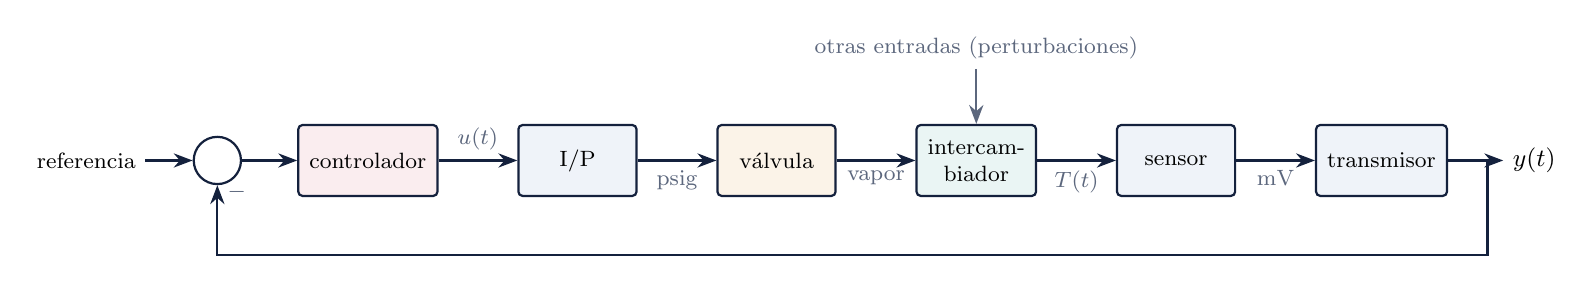
\begin{tikzpicture}[node distance=10mm, b/.style={bloque,minimum width=15mm,font=\footnotesize,align=center}]
  \node (r) {\footnotesize referencia};
  \node[suma,right=6mm of r] (S) {};
  \node[b,right=7mm of S,fill=ctrlcoral!10] (c) {controlador};
  \node[b,right=of c] (ip) {I/P};
  \node[b,right=of ip,fill=ctrlambar!12] (v) {válvula};
  \node[b,right=of v,fill=ctrlverde!10] (p) {intercam-\\biador};
  \node[b,right=of p] (se) {sensor};
  \node[b,right=of se] (tr) {transmisor};
  \coordinate[right=5mm of tr] (o); \node[right=2mm of o] (y) {$y(t)$};
  \node[above=7mm of p,font=\footnotesize,text=ctrlgris] (d) {otras entradas (perturbaciones)};
  \draw[senal] (r)--(S); \draw[senal] (S)--(c);
  \draw[senal] (c)--node[above,rot]{$u(t)$}(ip);
  \draw[senal] (ip)--node[below,rot]{psig}(v);
  \draw[senal] (v)--node[below,rot]{vapor}(p);
  \draw[senal] (p)--node[below,rot]{$T(t)$}(se);
  \draw[senal] (se)--node[below,rot]{mV}(tr);
  \draw[thick,draw=ctrlnoche] (tr)--(o); \draw[senal] (o)--(y);
  \draw[senal,draw=ctrlgris] (d)--(p);
  \draw[senal] (o)--++(0,-12mm) -| node[pos=0.95,right,rot]{$-$} (S);
\end{tikzpicture}
\end{document}
